\section{Arquitetura do Sistema}\label{systemarch}

%Antidote has a plug-in based architecture. So, a Castalia plugin was developed to support communication between Antidote Stack and Castalia Modules. As the Antidote is developed to work with real devices, modifications had to be made to the library to work in Castalia Simulator. The communication, encoders, agent and manager are some of the Antidote's modules modified.
A biblioteca Antidote é portátil e usa a linguagem ANSI-C para criar um código limpo e multi-plataforma. Para realizar a comunicação entre o Antidote e outros sistemas, como o Castalia, é necessário desenvolver e adaptar plug-ins de comunicação no Antidote que permitam essa comunicação. Assim, um Plug-in para o Simulador Castalia foi desenvolvido para intermediar a comunicação com a biblioteca Antidote. Como esta biblioteca foi desenvolvida para ser usada em dispositivos médicos reais, modificações foram necessárias para que o funcionamento dentro do simulador ocorresse como em um dispositivo real. Inúmeras partes do código foram alterados, como o gerenciamento de threads, porém, os principais módulos alterados foram: \textit{communication}, \textit{encoders}, \textit{agent} and \textit{manager}.

\subsection{Castalia Plugin}

%Antidote itself is portable and uses ANSI C language to create a standard and clean library. To provide a communication between Antidote and other systems, like Castalia, we must adapt and develop the necessary communication plug-ins.
A biblioteca Antidote suporta a utilização de plug-ins para prover comunicação com o ``mundo externo''. Esses plug-ins devem ser desenvolvidos e adaptados para que se estabeleça uma comunicação entre os dois sistemas. Um dos principais desafios no desenvolvimento deste plug-in, foi adaptar o Antidote, que é escrito em C, para funcionar no Castalia, que utiliza orientação a objetos em C++. 

%The proposed plug-in allows Castalia and Antidote to talk with each other through Castalia plug-in module. Inside Castalia, we can call any function from Antidote Library and retrieve any information from it, but transmitting data from Castalia to Antidote Library is not a simple task. To solve this, we first use external variables to make the data exchange between Castalia and Castalia plug-in module. Then, to obtain the data from Castalia plug-in module, Antidote uses pointers to Castalia plug-in functions that we call \textit{callback functions}. That is why we need a plug-in to mediate the communication.
O plug-in proposto permite que o Simulador Castalia e a biblioteca Antidote conversem entre si através de um módulo que chamamos de Castalia plug-in. Dentro do Castalia podemos chamar qualquer função da biblioteca Antidote e recuperar qualquer informação dela, mas transmitir os dados do Castalia para o Antidote não é uma tarefa simples. Para resolver isso, primeiro fazemos a troca de dados entre o módulo Castalia plug-in e o Simulador Castalia. Em seguida, para obter os dados do módulo Castalia plug-in, o Antidote usa ponteiros para funções do módulo Castalia plug-in, chamadas de \textit{callback functions}. É por isso que precisamos de um plug-in para mediar a comunicação.

%There is a set of callback functions in Castalia plug-in module that are passed to Antidote during the initialization process of each agent. These callback functions are passed to communication module of Antidote as pointers to functions. This way, whenever the communication module needs to retrieve or send a message, it just triggers the correspondent callback function. The task of these callback functions is to receive and send messages as also initialize and finalize a agent network.
Há um conjunto de \textit{callback functions} que são passadas para o Antidote durante o processo de inicialização de cada agente. Essas funções são passadas para o módulo de comunicação do Antidote como ponteiros para funções. Desta forma, sempre que o módulo de comunicação precisa recuperar ou enviar alguma mensagem, ele apenas aciona a \textit{callback function} correspondente.

%Figure~\ref{fig:CastaliaPlugin} depicts how Antidote gets messages from Castalia. The arriving messages are copied to an external variable in Castalia Simulator Module - the external variable is visible to both Castalia Simulator and Castalia Plugin module. Since the communication module in Antidote owns pointers to Castalia Plug-ins functions, it can retrieve the messages using callback functions.
A Figura \ref{fig:CastaliaPlugin} descreve como o Antidote recebe as mensagens do Castalia. As mensagens que chegam são copiadas para uma variável com escopo externo no Simulador Castalia - a variável externa é visível para os módulos do Castalia e Castalia Plug-in. Como o módulo de comunicação do Antidote possui ponteiros para as funções do módulo Castalia plug-in, ele pode recuperar as mensagens usando esses ponteiros (callback functions).

%\begin{figure}[htbp]
%\centerline{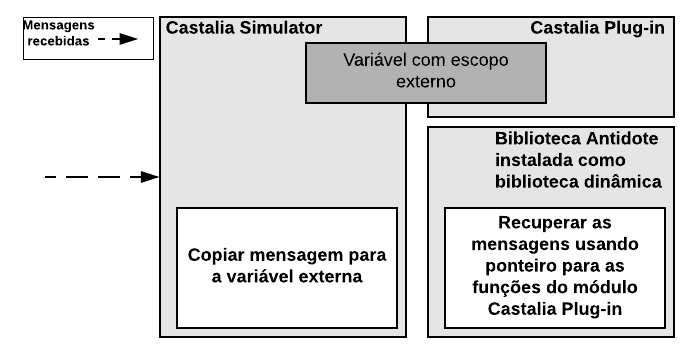
\includegraphics[scale=0.35]{figures/castaliaPlugin.png}}
%\caption{How Antidote Library gets messages from Castalia Simulator.}
%\label{fig:CastaliaPlugin}
%\end{figure}

\begin{figure}[ht]
\centering
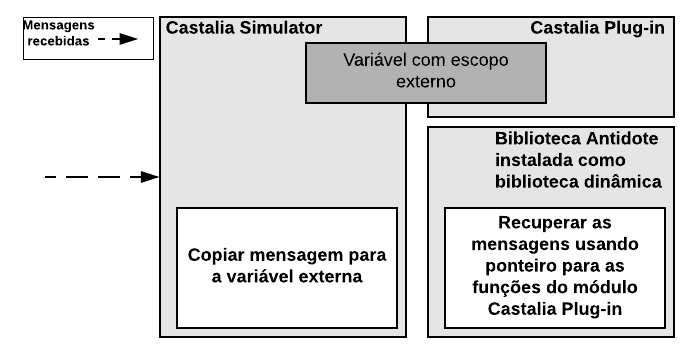
\includegraphics[width=.5\textwidth]{figures/castaliaPlugin.png}
\caption{How Antidote Library gets messages from Castalia Simulator}
\label{fig:CastaliaPlugin} 
\end{figure}

\subsection{Changes in communication module}

%The Communication module is one of the most important modules in the Antidote Library. The start, the end, transmissions, machine state phases of all nodes are controlled by this module. In a real scenario, each device has its own communication module, running its own copy of the code. But in a single-machine simulation, it is a bit different. Only one communication module has to handle all nodes, since the Antidote Library is installed in the operating system as a dynamic library.
O módulo de comunicação é um dos módulos mais importantes na biblioteca Antidote. A inicialização, a finalização, as fases da máquina de estados de todos os nós são controladas por este módulo. Em um cenário real, cada dispositivo possui seu próprio módulo de comunicação, executando sua própria cópia do código. Mas em uma simulação executada em uma única máquina é um pouco diferente. Somente um módulo de comunicação manipula todos os nós, uma vez que o Antidote é instalado no sistema operacional como uma biblioteca dinâmica.

%To ensure the proper operation of the Communication Module, the \textit{node id} is required in each function call, this way we know which node we are working with and apply the action for that node, without affecting other nodes. For example, if a node transits from unassociated state to associating machine state, without the proposed modification, this action would affect all nodes even those that should not change their machine states.
Para garantir o funcionamento adequado do módulo de comunicação, a identificação do nó é necessário em cada chamada de função, desta forma sabemos com qual nó estamos trabalhando e aplicamos a ação para apenas este nó, sem alterar o estado dos outros nós. Por exemplo, se um nó transitar do estado de máquina não associado para associando, sem a modificação proposta, essa ação afetaria todos os nós, mesmo aqueles que não deveriam alterar o estado de máquina. 

%Figure~\ref{fig:communicationModuleCastalia} illustrates the system modification. In every function in the Communication module, we insert the \textit{node id} new parameter. This way the communication module always knows the corresponding node. 
%The arrows in Fig.~\ref{fig:communicationModuleCastalia} represents functions calls.
A Figura \ref{fig:communicationModuleCastalia} ilustra a modificação do sistema. Em cada função do módulo de Comunicação, inserimos o novo parâmetro node id. Desta forma, o módulo de comunicação sempre conhece o nó em questão.

%\begin{figure}[htbp]
%\centerline{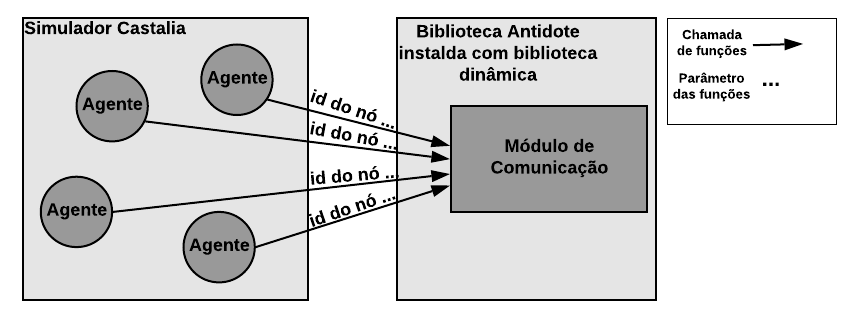
\includegraphics[scale=0.31]{figures/communicationModule.png}}
%\caption{Communication module handling several nodes. Each arrow represents a function being called from the Communication Module.}
%\label{fig:communicationModuleCastalia}
%\end{figure}

\begin{figure}[ht]
\centering
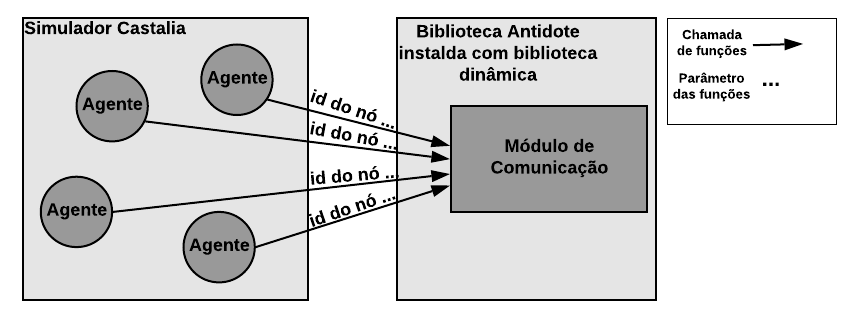
\includegraphics[width=.5\textwidth]{figures/communicationModule.png}
\caption{Communication module handling several nodes. Each arrow represents a function being called from the Communication Module}
\label{fig:communicationModuleCastalia} 
\end{figure}

\subsection{Other modifications}

%Other modules like Agent, Manager and Encoders were modified to smooth operation of Antidote functions in Castalia. We can highlight the function created in the encoder module to convert absolute values (the measurements) into scaled non-negative values as recommended by \cite{b1}. 
%Functions to finalize the Agents module were transferred to Manager module for the sake of simplicity and the \textit{node id} were add as a parameters of Agent and Manager functions. 
%In Encoder module a function to interpret the data received was created.
Outros módulos como Agent, Manager e Encoders foram modificados para facilitar o funcionamento das funções do Antidote para serem usados no Castalia. Podemos destacar a função criada no módulo do codificador para converter valores absolutos (as leituras) em valores não-negativos escalares, conforme recomendado por \cite{b1}. 

%It is useful to send absolute values like $-0.060$  which would require at least 4 bytes in X73-PHD floating point format to be sent. When converted, the number $-0.060$ becomes $388$, which requires just two bytes. The X73-PHD standard defines its own floating point types composed of a 32-bit word comprising a signed 8-bit integer exponent followed by a signed 24-bit integer mantissa.
%VINICIUS - acho melhor especificar pq falar só "many" fica muito genérico. R: feito.
Isso é útil para enviar valores absolutos como $-0.060$, o que exigiria pelo menos 4 bytes no formato de ponto flutuante da norma X73-PHD. Quando convertido, o número $-0.060$ torna-se 388, o que requer apenas dois bytes para ser enviado. O padrão X73-PHD define seus próprios tipos de ponto flutuante compostos por 32 bits que compreende um expoente inteiro com sinal de 8 bits seguido por uma mantissa de inteiro com sinal de 24 bits.

%Within the Manager, the equation to make the conversion from scaled to absolute values is given by expression\\$Y = M \times X + B$, where:
No gerente, a equação para fazer a conversão dos valores escalares para valores absolutos é dada pela expressão Y = M × X + B, onde:
\begin{align*}
    Y &= \text{valor absoluto}\\
    M &= \frac{(\text{maior valor absoluto} - \text{menor valor absoluto})}{(\text{maior valor escalar} - \text{menor valor escalar})}\\
    B &= \text{maior valor absoluto} - (M \times \text{maior valor escalar})\\
    X &= \text{valor escalar}
\end{align*}

%Within an Agent, the conversion from absolute values to scaled values is given by expression $X = \frac{(R - B)}{M}$, where: $R =$ actual measured value.
No agente, a conversão de valores absolutos para valores escalares é dada pela expressão $X = \frac{(R - B)}{M}$, onde:
\begin{align*}
   R &= \text{valor atual da leitura (valor absoluto)}
\end{align*}

%A thermometer that does readings from $-45^\circ$C  to $50^\circ$C with a resolution of $0.5^\circ$C has the following values: lower absolute value = $-45.0$, upper absolute value = $50.0$, lower scaled value = $0$, upper scaled value = $190$. Giving $M = 0.5$ and $B = -45.0$.
Um termômetro que faz leituras de $-45^\circ$C até $50^\circ$C com uma resolução de $0.5^\circ$C tem os seguintes valores:

\begin{align*}
    \text{Menor valor absoluto} &= -45.0 \\
    \text{Maior valor absoluto} &= 50.0 \\
    \text{Menor valor escalar} &= 0 \\
    \text{Maior valor escalar} &= 190
\end{align*}

%Giving $M = \frac{(50.0 - (-45.0))}{(190 – 0)} = 0.5$ and $B = 50.0 - (0.5 \times 190) = -45.0$

%The Castalia plug-in module and the modifications to Antidote Library were made exclusively for WBAN simulation in Castalia.
O módulo Castalia plug-in e as modificações na biblioteca Antidote foram feitas apenas para simulações de WBAN no Simulador Castalia. Nenhum teste foi feito em outro simulador.

%VINICIUS - talvez uma conclusão dessa seção fosse inteiressante, R: Feito